

\subsection{GUI}

Our GUI is a template and AJAX based web application. It utilizes Django's
template system to implement the View part of the MVC principle. 

Each webpage is a template populated through Python code before it is delivered
to the webserver and ultimately the requesting web browser.

Additional data that needs delivered to a web page, say if the user interacts
with the GUI, the additional data is requested through Javascript and AJAX
calls and then get's added to the already loaded DOM in the web browser.

\subsubsection{Structure}

The pages of the GUI is organized in the following structure.

\begin{figure}[ht!]
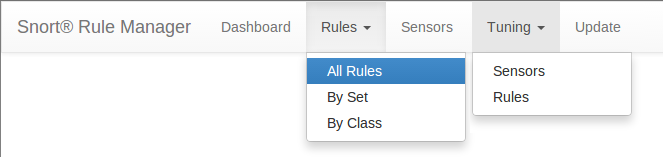
\includegraphics[width=130mm]{./img/gui_structure.png}
\caption{GUI Structure}
\label{gui_structure}
\end{figure}

\subsubsection{Design}

The GUI is designed with simplicity in mind and we achieved this using a
front-end framework called Bootstrap. This framework gave us easy to use and
ready made design elements for HTML and CSS, saving us time and energy. 

So instead of creating a <table> element and spending hours setting up and
tweaking the CSS for said table element, we could just add <table class=`{\bf
table table-bordered}`> and get the table formatted nicely with colors and fonts
that are typographically matching.

\subsubsection{Features}
\paragraph{Content Prefetching}
One of the main features of our GUI design is our usage of prefetching to speed
up loading. Instead of loading absolutely everything into the web browsers DOM,
like our predecessor BHTB did, we instead initially only load the first page or
page elements. This significantly reduces loading times.

We then silently in the background load in any element the user might want to
see next, through AJAX calls. When the user then interacts with the GUI, the
next elements are shown to the user. The next-next elements are also loaded
through AJAX calls so that they are ready.

This ensures that the user always has immidiate response from any interaction
done with the GUI, while keeping loading times to a bare minimum.

\subsubsection{Rules/All rules page}

\begin{figure}[ht!]
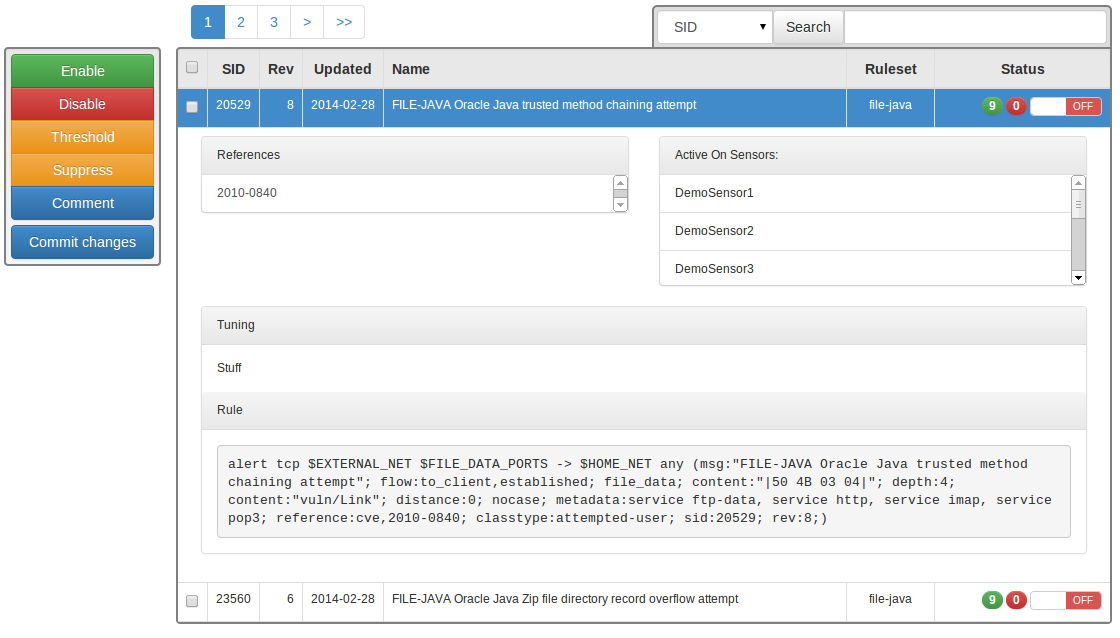
\includegraphics[width=150mm]{./img/gui_rules_allrules.png}
\caption{Rules/All rules page}
\label{gui_rules_allrules}
\end{figure}

This page serves as the complete list of all rules currently residing in the
central database. Because the central database can literally contain hundreds of
thousands of rules, this list is paginated. Pages are loaded using AJAX calls to
prefetch them as needed.

Each row in the list can be clicked on, which expands an area containing
additional information about the rule in question. 

We anticipate that the main use of this page is to utilize the search function
to find a specific rule or rules and then either retrieve information about them
or tune them.

Rules can be tuned by checking the checkbox associated with the rule in question
and then press the button that represent the desired function in the box to the
left. 

